\chapter{Anhang}

\begin{figure}
	\centering
	\begin{subfigure}{0.48\textwidth}
		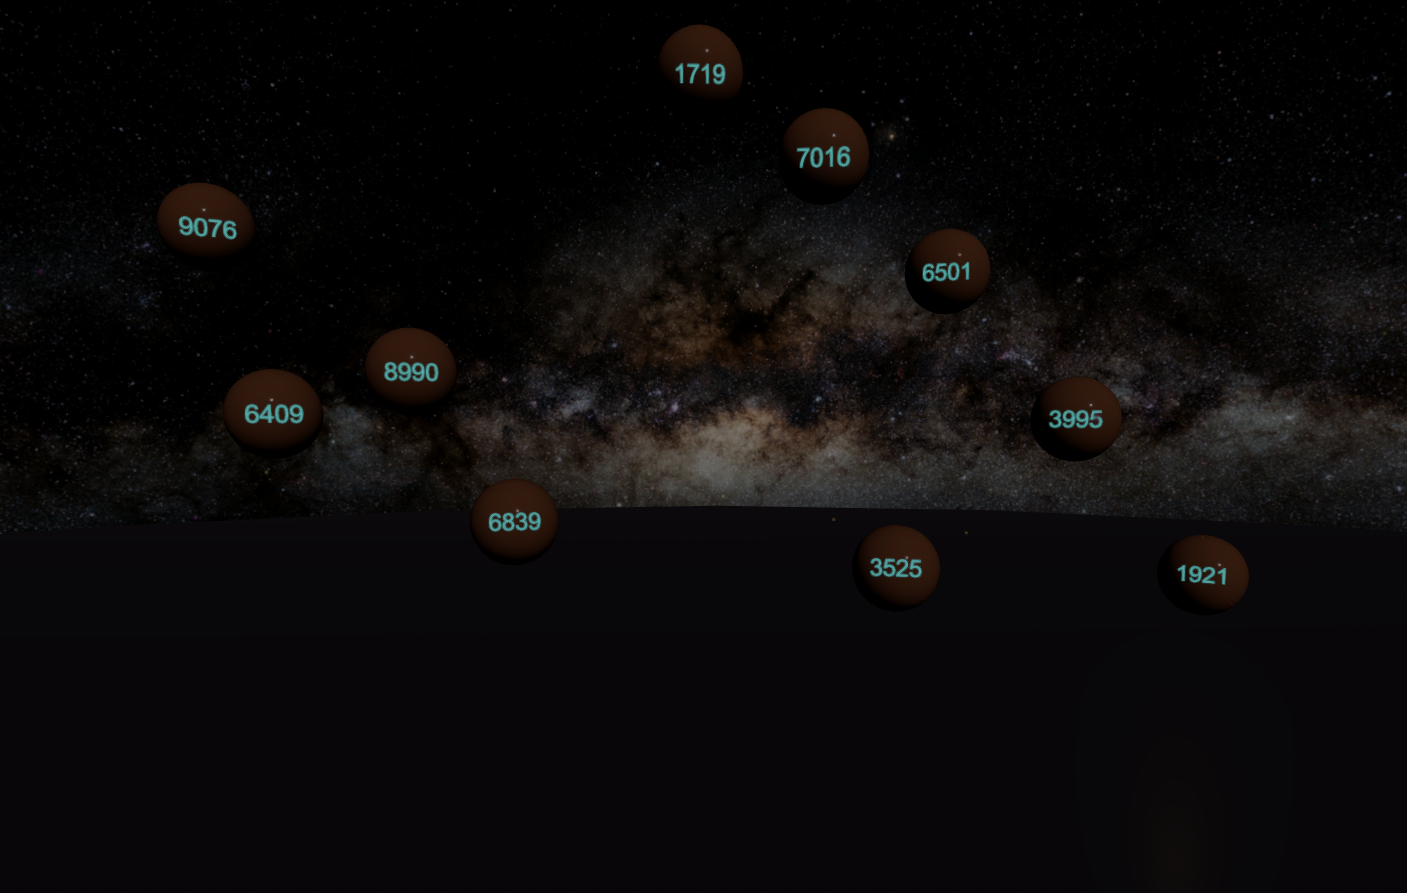
\includegraphics[width=\textwidth]{./images/ordering.png}
		\caption{Erste Aufgabe der Studie.}
		\label{fig:ordering}
	\end{subfigure}%
	\hfill
	\begin{subfigure}{0.48\textwidth}
		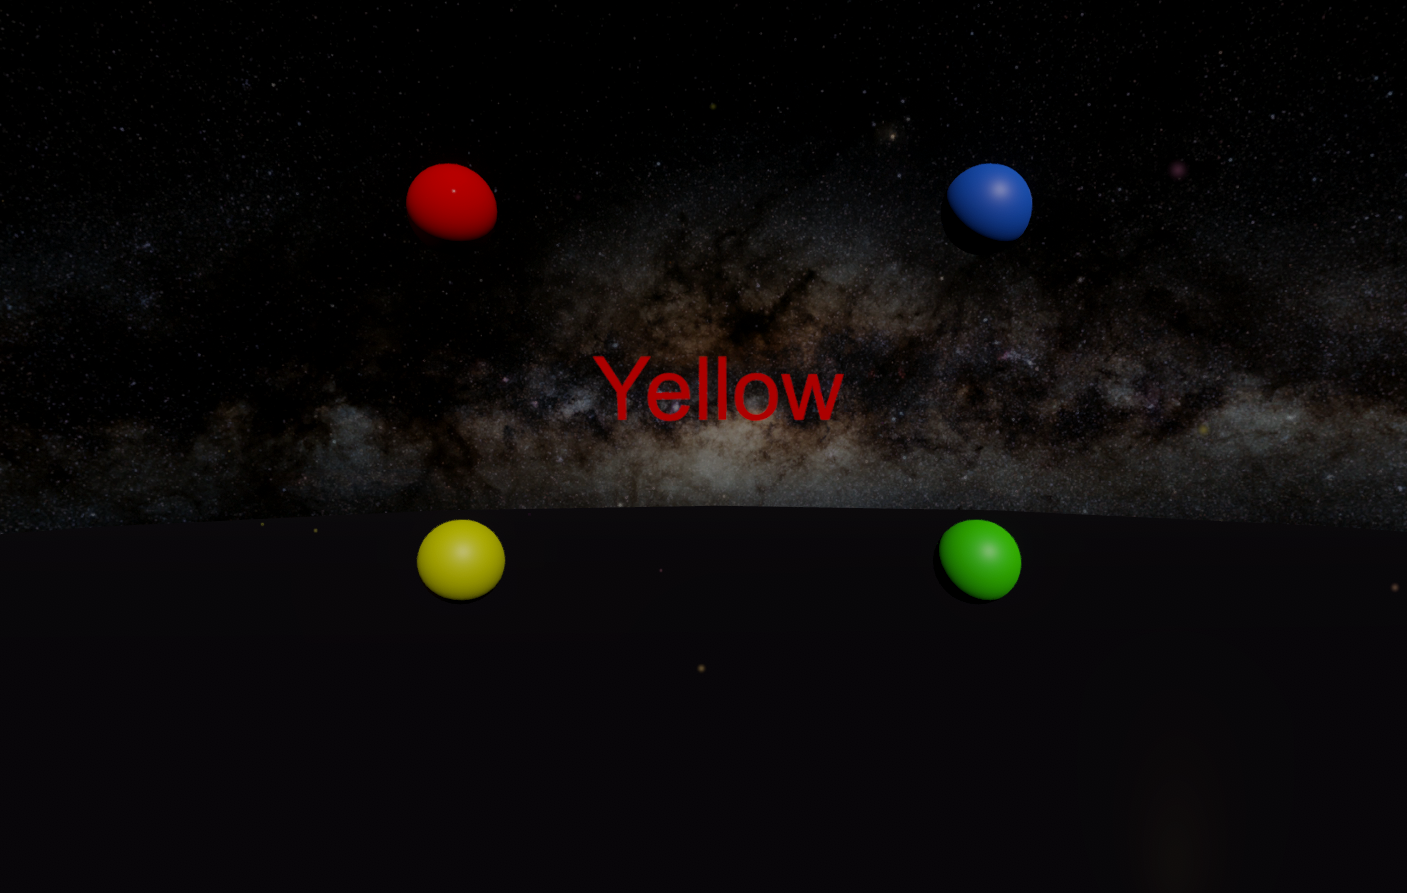
\includegraphics[width=\textwidth]{./images/matching.png}
		\caption{Zweite Aufgabe.}
		\label{fig:matching}
	\end{subfigure}
	\hfill
	\begin{subfigure}{0.48\textwidth}
		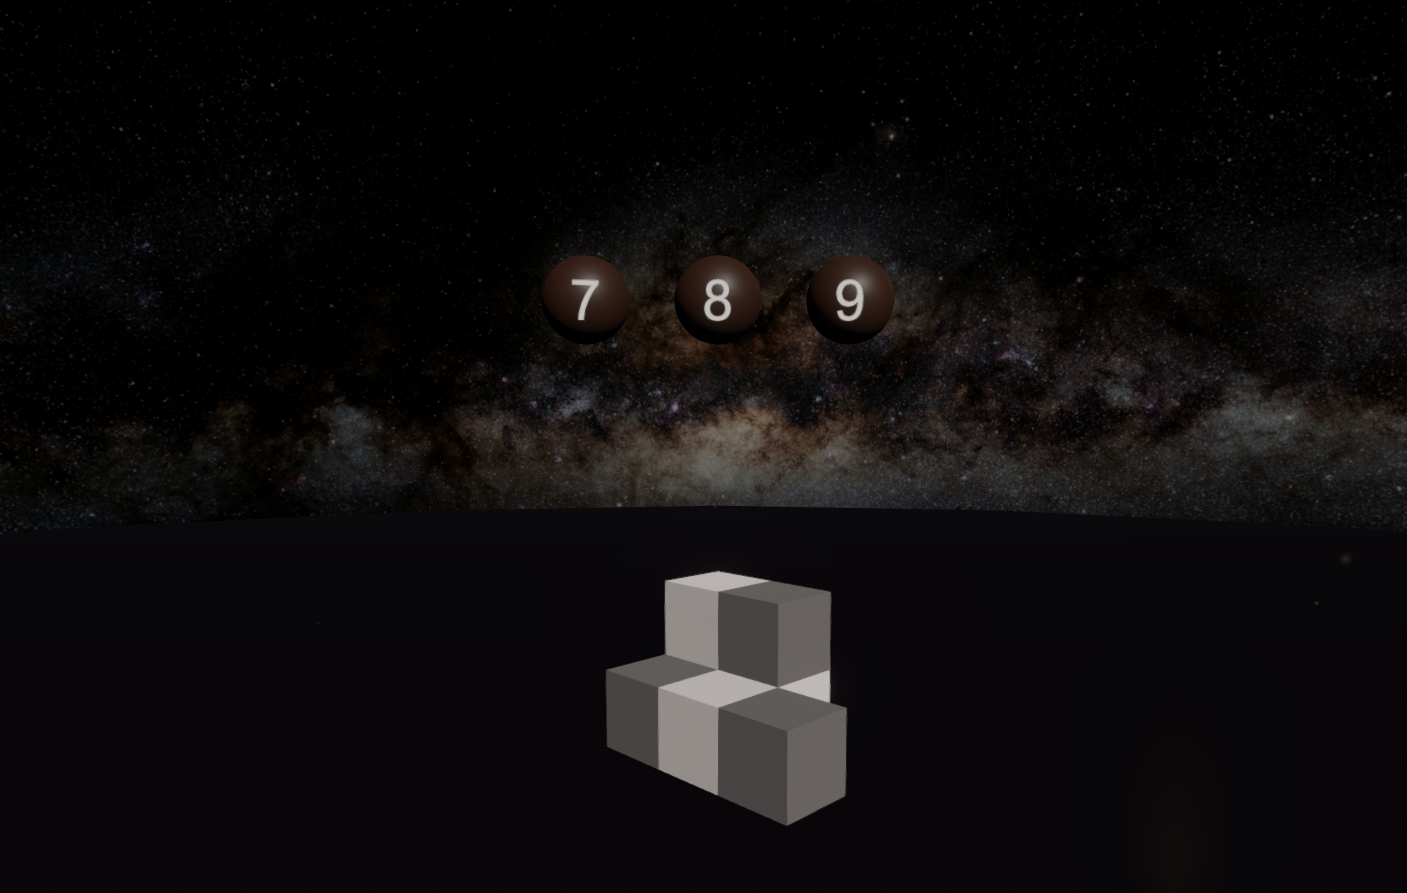
\includegraphics[width=\textwidth]{./images/counting.png}
		\caption{Dritte Aufgabe in der Studie.}
		\label{fig:counting}
	\end{subfigure}
	\caption{Screenshots für die Aufgaben mit denen die Teilnehmer der Studie konfrontiert werden.} % caption for whole figure
\end{figure}

\begin{table*}
	\caption{Numerische Auflistung der Ergebnisse der Frage "`Please select your gender"'.}~\label{tab:sc_results_gender}
	
	\setlength\tabcolsep{3pt}
	\renewcommand{\arraystretch}{1.4}% for the vertical padding
	\begin{tabularx}{\textwidth}{ | x || r | r | }
		\hline
		Geschlecht & Absolutwerte 	& Prozentwerte \\ \hline\hline
		Männlich & 33 & 73.3\% \\ \hline
		Weiblich & 12 & 26.7\% \\ \hline
		Divers & 0 & 0.0\% \\ \hline
	\end{tabularx}
\end{table*}

\begin{table*}
	\caption{Numerische Statistik der Ergebnisse der Frage "`Please enter your age in years"'.}~\label{tab:sc_results_age}
	
	\setlength\tabcolsep{3pt}
	\renewcommand{\arraystretch}{1.4}% for the vertical padding
	\begin{tabularx}{\textwidth}{ | x | x | x | x | x | x | }
		\hline
		Min & Max & Range & Median & Mean  & Standard Deviation \\ \hline\hline
		19  & 30  & 11    & 23     & 23.04 & 2.53              \\ \hline
	\end{tabularx}
\end{table*}

\begin{table*}
	\caption{Verteilung der Antworten zur Frage "`How much experience do you have with VR?"'.}~\label{tab:sc_results_expVR}
	
	\setlength\tabcolsep{3pt}
	\renewcommand{\arraystretch}{1.4}% for the vertical padding
	\begin{tabularx}{\textwidth}{ | x || r | r | }
		\hline
		Studienfach 						& Absolutwerte 	& Prozentwerte \\ \hline\hline
		[A1] No experience at all 			& 10 			& 22.2\% \\ \hline
		[A2] Almost no experience 			& 15 			& 33.3\% \\ \hline
		[A3] Less than average experience 	& 3 			& 6.7\% \\ \hline
		[A4] Some experience 				& 10 			& 22.2\% \\ \hline
		[A5] More than average experience 	& 2 			& 4.4\% \\ \hline
		[A6] Experienced 					& 2 			& 4.4\% \\ \hline
		[A7] Very highly experienced 		& 3 			& 6.7\% \\ \hline
	\end{tabularx}
\end{table*}

\begin{table*}
	\caption{Numerische Statistik der Ergebnisse der Frage "`How much experience do you have with VR?"'.}~\label{tab:sc_numbers_expVR}
	
	\setlength\tabcolsep{3pt}
	\renewcommand{\arraystretch}{1.4}% for the vertical padding
	\begin{tabularx}{\textwidth}{ | x | x | x | x | x | x | }
		\hline
		Min & Max & Range & Median & Mean  & Standard Deviation \\ \hline\hline
		1  & 7  & 6    & 2     & 2.93 & 1.78              \\ \hline
	\end{tabularx}
\end{table*}

\begin{table*}
	\caption{Verteilung der Antworten zur Frage "`How much experience do you have with AR?"'.}~\label{tab:sc_results_expAR}
	
	\setlength\tabcolsep{3pt}
	\renewcommand{\arraystretch}{1.4}% for the vertical padding
	\begin{tabularx}{\textwidth}{ | x || r | r | }
		\hline
		Studienfach 						& Absolutwerte 	& Prozentwerte \\ \hline\hline
		[A1] No experience at all 			& 17 			& 37.7\% \\ \hline
		[A2] Almost no experience 			& 10 			& 22.2\% \\ \hline
		[A3] Less than average experience 	& 7 			& 15.5\% \\ \hline
		[A4] Some experience 				& 8 			& 17.7\% \\ \hline
		[A5] More than average experience 	& 2 			& 4.4\% \\ \hline
		[A6] Experienced 					& 1 			& 2.2\% \\ \hline
		[A7] Very highly experienced 		& 0 			& 0.0\% \\ \hline
	\end{tabularx}
\end{table*}

\begin{table*}
	\caption{Numerische Statistik der Ergebnisse der Frage "`How much experience do you have with AR?"'.}~\label{tab:sc_numbers_expAR}
	
	\setlength\tabcolsep{3pt}
	\renewcommand{\arraystretch}{1.4}% for the vertical padding
	\begin{tabularx}{\textwidth}{ | x | x | x | x | x | x | }
		\hline
		Min & Max & Range & Median & Mean  & Standard Deviation \\ \hline\hline
		1  & 6  & 5    & 2     & 2.36 & 1.38              \\ \hline
	\end{tabularx}
\end{table*}

\begin{table*}
	\caption{Verteilung der Antworten zur Frage "`What subject, if any, did you study or are you currently studying?"'.}~\label{tab:sc_results_study}
	
	\setlength\tabcolsep{3pt}
	\renewcommand{\arraystretch}{1.4}% for the vertical padding
	\begin{tabularx}{\textwidth}{ | x || r | r | }
		\hline
		Studienfach & Absolutwerte & Prozentwerte \\ \hline\hline
		Biologie & 1 & 2.2\% \\ \hline
		Informatik & 8 & 17.8\% \\ \hline
		Informationssystemtechnik & 1 & 2.2\% \\ \hline
		Mathematik & 1 & 2.2\% \\ \hline
		Medieninformatik & 18 & 40.0\% \\ \hline
		Physik & 3 & 6.7\% \\ \hline
		Psychologie & 2 & 4.4\% \\ \hline
		Software Engineering & 8 & 17.8\% \\ \hline
		Wirtschaftsmathematik & 1 & 2.2\% \\ \hline
		Wirtschaftsphysik & 2 & 4.4\% \\ \hline
	\end{tabularx}
\end{table*}

\begin{table*}
	\caption{Verteilung der Einstellungen des Stuhls. Die Teilnehmer können die Rückenlehne nach ihren persönlichen Präferenzen neigen.}~\label{tab:sc_results_chair}
	
	\setlength\tabcolsep{3pt}
	\renewcommand{\arraystretch}{1.4}% for the vertical padding
	\begin{tabularx}{\textwidth}{ | x || r | r | }
		\hline
		Winkeleinstellungen	in Grad	& Absolutwerte 	& Prozentwerte \\ \hline\hline
		0 							& 7 			& 15.6\% \\ \hline
		30 							& 23			& 51.1\% \\ \hline
		60	 						& 10 			& 22.2\% \\ \hline
		90							& 5 			& 11.1\% \\ \hline
	\end{tabularx}
\end{table*}

\begin{itemize}
	\captionof{anno}{Anmerkungen und Hinweise von Studienteilnehmern}\label{lis:comments}
	\item "`Die Musik war sehr störend, um in einen Ruhezustand zu kommen"'
	\item "`Die VR Umgebung war schön gestaltet, aber die rumschwebenden Partikel waren eher verwirrend, ich dachte ich kann mit diesen interagieren"'
	\item "`Der Stuhl war sehr entspannend und bequem"'
	\item "`Es fiel mir schwer einzuschlafen, da ich zum 1. mal VR gemacht habe und dann neugierig war"'
	\item "`Die Musik war sehr angenehm"'
	\item "`Das lange gedrückt halten zur Interaktion war störend"'
	\item "`haptisches Feedback durch Controller wäre gut gewesen"'
	\item "`Die Brille war sehr unangenehm"'
	\item "`Der Ton fürs Wecken hat mich erschrocken"'
	\item "`Mit meiner Brille war es unangenehm die VR Brille zu tragen"'
	\item "`Ich konnte mich sehr gut entspannen, richtig eingeschlafen bin ich      aber nicht"'
	\item "`Die Interaktion mit dem Controller war sehr intuitiv"'
	\item "`Mir kam die Zeit zum entspannen deutlich länger als 15 Minuten vor "'
	\item "`Egal wie ich die Brille verstellte, richtig scharf konnte ich nie sehen "'
	\item "`Noch fünf bis zehn Minuten länger und ich wäre komplett eingeschlafen "'
\end{itemize}

\begin{table*}
	\caption{Wahrgenommene Schlafdauer als subjektive Aussage der Studienteilnehmer.}~\label{tab:sleepduration}
	
	\setlength\tabcolsep{3pt}
	\renewcommand{\arraystretch}{1.4}% for the vertical padding
	\begin{tabularx}{\textwidth}{ | x || r | r | }
		\hline
		wahrgenommene Schlafdauer in min & Absolutwerte & Prozentwerte \\ \hline\hline
		8						   	     & 2			   & 4.4\% \\ \hline
		10   					         & 5			   & 11.1\% \\ \hline
		11						   	     & 1 		   & 2.2\% \\ \hline
		12						   	     & 3			   & 6.7\% \\ \hline
		13							     & 2			   & 4.4\% \\ \hline
		14							     & 1			   & 2.2\% \\ \hline
		10-15	      					 & 3		 & 6.7\% \\ \hline
		15							     & 13		 & 28.9\% \\ \hline
		15-20							 & 1		 & 2.2\% \\ \hline
		17								 & 2		 & 4.4\% \\ \hline
		18								 & 3		 & 6.7\% \\ \hline
		18,5							 & 1		 & 2.2\% \\ \hline
		19								 & 1		 & 2.2\% \\ \hline
		20								 & 6		 & 13.3\% \\ \hline
		30								 & 1		 & 2.2\% \\ \hline
	\end{tabularx}
\end{table*}

\begin{table*}
	\caption{Numerische Statistik der Ergebnisse zur empfundenen Schlafdauer.}~\label{tab:sc_numbers_expAR}
	
	\setlength\tabcolsep{3pt}
	\renewcommand{\arraystretch}{1.4}% for the vertical padding
	\begin{tabularx}{\textwidth}{ | x | x | x | x | x | x | }
		\hline
		Min & Max & Range & Median & Mean  & Standard Deviation \\ \hline\hline
		8  & 30  & 22    & 15     & 15.08 & 4.10              \\ \hline
	\end{tabularx}
\end{table*}

\begin{table*}
	\caption{Verteilung der Antworten zur Frage "`Hast du geschlafen?"' .}~\label{tab:sleepstatus}
	
	\setlength\tabcolsep{3pt}
	\renewcommand{\arraystretch}{1.4}% for the vertical padding
	\begin{tabularx}{\textwidth}{ | x || r | r | }
		\hline
		Schlafmodus					& Absolutwerte 	& Prozentwerte \\ \hline\hline
		geschlafen 					& 9 			& 20.0\% \\ \hline
		gedöst/kurz vor eingeschlafen	& 12			& 26.7\% \\ \hline
		meditiert					& 3			& 6.7\% \\ \hline
		nicht geschlafen			& 21 			& 46.7\% \\ \hline
	\end{tabularx}
\end{table*}

\begin{table*}
	\caption{Numerische Statistik der Ergebnisse der Frage "`Please estimate your mental effort for the previous tasks"'.}~\label{tab:sc_results_rsme}
	
	\setlength\tabcolsep{3pt}
	\renewcommand{\arraystretch}{1.4}% for the vertical padding
	\begin{tabularx}{\textwidth}{ | x | x | x | x | x | x | }
		\hline
		Min & Max & Range & Median & Mean  & Standard Deviation \\ \hline\hline
		0.13  & 0.66  & 0.53    & 0.27     & 0.28 & 0.11              \\ \hline
	\end{tabularx}
\end{table*}

\begin{table*}
	\caption{Statistik der Dauer des Alarm-Tons. Die Zeitmessung startet sobald die Schlafphase endet und der Alarm ertönt und endet mit Bestätigung durch den Benutzer.}~\label{tab:times_results_alarm}
	
	\setlength\tabcolsep{3pt}
	\renewcommand{\arraystretch}{1.4}% for the vertical padding
	\begin{tabularx}{\textwidth}{ | x | x | x | x | x | x | }
		\hline
		Min   & Max   & Range & Median  & Mean   & Standard Deviation \\ \hline\hline
		3.91  & 10.84 & 6.93  & 5.87    & 6.60   & 2.18               \\ \hline
	\end{tabularx}
\end{table*}

\begin{table*}
	\caption{Statistik der Fehler der Aufgaben unterteilt sowohl nach Aufgabe als auch nach Gruppe.}~\label{tab:sc_results}
	
	\setlength\tabcolsep{3pt}
	\renewcommand{\arraystretch}{1.4}% for the vertical padding
	\begin{tabularx}{\textwidth}{ | l | x | x | x | x | x | x | }
		\hline
		Gruppe & Min   & Max   & Range & Median  & Mean   & Standard Deviation  \\ \hline\hline
		\multicolumn{7}{| l |}{ Aufgabe 1: Zahlenfolge } 						\\ \hline
		Alarm   & 0 & 45 & 45 & 0 & 10.50 & 18.10 \\ \hline
		Fade 20 & 0 & 13 & 13 & 1 & 1.87 & 3.46 \\ \hline
		Fade  5 & 0 & 2 & 2 & 0 & 0.40 & 0.74 \\ \hline
		\multicolumn{7}{| l |}{ Aufgabe 2: Stroop-Effekt } 						\\ \hline
		Alarm   & 0 & 9 & 9 & 0 & 1.20 & 2.83 \\ \hline
		Fade 20 & 0 & 10 & 10 & 0 & 1.50 & 3.10 \\ \hline
		Fade  5 & 0 & 9 & 9 & 0 & 1.20 & 2.83 \\ \hline
		\multicolumn{7}{| l |}{ Aufgabe 3: Boxen zählen } 						\\ \hline
		Alarm   & 0 & 1 & 1 & 0 & 0.33 & 0.49 \\ \hline
		Fade 20 & 0 & 2 & 2 & 0 & 0.33 & 0.72 \\ \hline
		Fade  5 & 0 & 2 & 2 & 0 & 0.27 & 0.59 \\ \hline
	\end{tabularx}
\end{table*}

\begin{table*}
	\caption{Vorkommnisse der Fehler unterteilt in Gruppen in Aufgabe 1: Zahlenfolge.}~\label{tab:orderingMistakeNumbers}
	
	\setlength\tabcolsep{3pt}
	\renewcommand{\arraystretch}{1.4}% for the vertical padding
	\begin{tabularx}{\textwidth}{ | l | x | x | x | x | x | x | x | x | x | }
		\hline
		Anzahl Fehler & 0   & 1  & 2  & 4  & 6  & 13 & 17 & 44  & 45 \\ \hline\hline
		Alarm 	  & 8  & 1  & 1  & 1  & 0  & 0  & 1  &  2  & 1  \\ \hline
		Fade 20	  & 7  & 3  & 3  & 0  & 1  & 1  & 0  &  0  & 0  \\ \hline
		Fade 5	  & 11  & 2  & 2  & 0  & 0  & 0  & 0  &  0  & 0  \\ \hline
	\end{tabularx}
\end{table*}

\begin{table*}
	\caption{Vorkommnisse der Fehler unterteilt in Gruppen in Aufgabe 2: Stroop-Effekt.}~\label{tab:matchingMistakeNumbers}
	
	\setlength\tabcolsep{3pt}
	\renewcommand{\arraystretch}{1.4}% for the vertical padding
	\begin{tabularx}{\textwidth}{ | l | x | x | x | x | x | x | x | }
		\hline
		Anzahl Fehler & 0   & 1  & 2  & 7  & 8  & 9 & 10 \\ \hline\hline
		Alarm 	  & 12  & 0  & 1  & 1  & 0  & 1 & 0  \\ \hline
		Fade 20   & 9  & 4  & 0  & 0  & 1  & 0 & 1  \\ \hline
		Fade 5 	  & 12  & 0  & 1  & 1  & 0  & 1 & 0  \\ \hline
	\end{tabularx}
\end{table*}

\begin{table*}
	\caption{Vorkommnisse der Fehler in Aufgabe 3: Boxen zählen.}~\label{tab:countingMistakeNumbers}
	
	\setlength\tabcolsep{3pt}
	\renewcommand{\arraystretch}{1.4}% for the vertical padding
	\begin{tabularx}{\textwidth}{ | l | x | x | x | }
		\hline
		Anzahl Fehler & 0   & 1  & 2 \\ \hline\hline
		Alarm 	  & 10  & 5  & 0 \\ \hline
		Fade 20   & 12  & 1  & 2 \\ \hline
		Fade 5 	  & 12  & 2  & 1 \\ \hline
	\end{tabularx}
\end{table*}

\begin{table*}
	\caption{Statistik der Dauer bis zur endgültigen Erledigung der Aufgaben (in Sekunden) unterteilt nach Aufgabe und nach Gruppe. Die Zeitmessung startet mit der Bestätigung durch den Benutzer und endet mit der Erledigung der Aufgabe.}~\label{tab:times_results}
	
	\setlength\tabcolsep{3pt}
	\renewcommand{\arraystretch}{1.4}% for the vertical padding
	\begin{tabularx}{\textwidth}{ | l | x | x | x | x | x | x | }
		\hline
		Gruppe & Min   & Max   & Range & Median  & Mean   & Standard Deviation  \\ \hline\hline
		\multicolumn{7}{| l |}{ Aufgabe 1: Zahlenfolge } 						\\ \hline
		Alarm  & 19.01 & 37.60 & 18.59 & 23.35   & 25.79  & 5.91                \\ \hline
		Fade 20 & 18.45 & 37.52 & 19.07 & 25.96   & 27.35  & 5.30               \\ \hline
		Fade  5 & 16.59 & 43.49 & 26.90 & 26.99   & 27.26  & 7.63               \\ \hline
		\multicolumn{7}{| l |}{ Aufgabe 2: Stroop-Effekt } 						\\ \hline
		Alarm  & 13.87 & 32.16 & 18.30 & 19.99   & 22.02  & 6.06                \\ \hline
		Fade 20 & 17.67 & 83.31 & 65.64 & 21.79   & 25.78  & 16.18               \\ \hline
		Fade  5 & 16.43 & 48.86 & 32.43 & 20.90   & 24.88  & 9.08               \\ \hline
		\multicolumn{7}{| l |}{ Aufgabe 3: Boxen zählen } 						\\ \hline
		Alarm  & 15.34 & 52.65 & 37.32 & 31.72   & 32.07  & 9.48                \\ \hline
		Fade 20 & 21.41 & 53.85 & 32.43 & 33.54   & 32.71  & 8.23               \\ \hline
		Fade  5 & 19.37 & 54.15 & 34.79 & 29.34   & 33.47  & 11.52               \\ \hline
	\end{tabularx}
\end{table*}

\begin{table*}
	\caption{Median der Zeiten der Unteraufgaben in einzelnen Aufgaben (in Sekunden). Die Zeiten geben an, welche zeit zwischen den einzelnen Unteraufgaben vergangen ist, entsprechen also der Verarbeitungszeit von einer Entscheidung zur Nächsten. \{S1:S10\} gibt hierbei die jeweilige Unteraufgabe an.}~\label{tab:times_subtasks}
	
	\setlength\tabcolsep{3pt}
	\renewcommand{\arraystretch}{1.4}% for the vertical padding
	\begin{tabularx}{\textwidth}{ | l | x | x | x | x | x | x | x | x | x | x | }
		\hline
		Gruppe 	& S1 & S2 & S3 & S4 & S5 & S6 & S7 & S8 & S9 & S10 \\ \hline\hline
		\multicolumn{11}{| l |}{ Aufgabe 1: Zahlenfolge } 			\\ \hline
		Alarm 	& 5.16 & 1.91 & 4.38 & 1.54 & 3.52 & 1.39 & 1.47 & 1.29 & 1.02 & 0.82 \\ \hline
		Fade 20 & 5.45 & 2.47 & 3.96 & 2.09 & 3.54 & 1.68 & 1.93 & 1.87 & 1.28 & 0.97 \\ \hline
		Fade 5  & 6.03 & 2.83 & 4.46 & 1.68 & 4.80 & 1.31 & 1.43 & 1.38 & 1.03 & 0.87 \\ \hline	
		\multicolumn{11}{| l |}{ Aufgabe 2: Stroop-Effekt } 				\\ \hline
		Alarm 	& 2.94 & 1.88 & 2.08 & 1.94 & 1.74 & 1.72 & 1.63 & 1.81 & 1.79 & 1.68 \\ \hline
		Fade 20 & 3.07 & 2.38 & 1.81 & 2.02 & 2.01 & 1.81 & 1.81 & 1.78 & 1.70 & 1.83 \\ \hline
		Fade 5  & 4.13 & 2.10 & 1.98 & 2.21 & 1.89 & 1.79 & 1.97 & 1.58 & 1.71 & 1.78 \\ \hline	
		\multicolumn{11}{| l |}{ Aufgabe 3: Boxen zählen } 					\\ \hline
		Alarm 	& 8.81 & 9.54 & 10.16 & - & - & - & - & - & - & - \\ \hline
		Fade 20 & 9.89 & 10.41 & 8.79 & - & - & - & - & - & - & - \\ \hline
		Fade 5  & 9.97 & 9.98 & 9.38  & - & - & - & - & - & - & - \\ \hline
	\end{tabularx}
\end{table*}
